\newpage
\section{Процесс загрузки приложений в Linux}

\subsection{ELF -- формат исполнения и компоновки}

Изначально UNIX (и производные от нее операционные системы) поддерживали множество исполняемых форматов, но теперь стандартом де-факто для LINUX и BSD стал ELF. Стандарт для формата ELF изначально был разработан и опубликован компанией USL как часть двоичного интерфейса приложений операционной системы UNIX System V. Затем он был выбран комитетом TIS и развит в качестве переносимого формата для различных операционных систем, работающих на 32-разрядной аппаратной архитектуре Intel x86. ELF быстро набрал популярность и, после того как компания HP расширила формат и опубликовала стандарт ELF-64, распространился и на 64-разрядных платформах. Иногда еще встречается древний a.out, но это достаточно особые случаи, требующие совместимости с железом.

Аббревиатура ELF расшифровывается как Execution and Linkable Format (формат исполнения и компоновки). Он во многом напоминает win32 PE. В начале ELF-файла расположен служебный заголовок (ELF-header), описывающий основные характеристики файла — тип (исполнения или линковки), архитектура ЦП, виртуальный адрес точки входа, размеры и смещения остальных заголовков…

За ELF-header'ом следует таблица сегментов (program header table), перечисляющая имеющиеся сегменты и их атрибуты. В формате линковки она необязательно. Линкеру сегменты не важны и он работает исключительно на уровне секций. Напротив, системный загрузчик, загружающий исполняемый ELF-файл в память, игнорирует секции, и оперирует целыми сегментами\cite{Cit1}.

Стандарт формата ELF различает несколько типов файлов:
\begin{itemize}
\item Перемещаемый файл -- хранит инструкции и данные, которые могут быть связаны с другими объектными файлами. Результатом такой связи может быть разделяемый объектный файл или исполняемый файл. К этому типу относятся объектные файлы статических библиотек.
\item Разделяемый объектный файл -- также содержит инструкции и данные и может быть связан с другими перемещаемыми файлами и разделяемыми объектными файлами, в результате чего будет создан новый объектный файл, либо при запуске программы на выполнение операционная система может динамически связать его с исполняемым файлом программы, в результате чего будет создан исполняемый образ программы. В последнем случае речь идет о разделяемых библиотеках.
\item Исполняемый файл -- содержит полное описание, позволяющее системе создать образ процесса. В том числе: инструкции, данные, описание необходимых разделяемых объектных файлов и необходимую символьную и отладочную информацию.
\end{itemize}

\subsection{Сегменты и секции}

Сегмент -- это непрерывная область адресного пространства со своими атрибутами доступа. В частности, сегмент кода имеет атрибут исполнения, а сегмент данных -- атрибуты чтения и записи. Стоит отметить, что ELF-сегменты это не сегменты x86 процессора! В защищенном режиме 386+ никаких "сегментов" уже нет, а есть только селекторы и все сегменты ELF-файла загружается в единый 4 Гбайтовый x86-сегмент! В зависимости от типа сегмента, величина выравнивания в памяти может варьировать от 4h до 1000h байт (размер страницы на x86). В самом ELF-файле хранятся в невыровненном виде, плотно прижатые друг к другу.

Ближайший аналог ELF-сегментов -- PE-секции, но в PE-файлах, секция -- это наименьшая структурная единица, а в ELF-файлах сегмент может быть разбит на один или несколько фрагментов -- секций. В частности, типичный кодовый сегмент состоит из
\begin{itemize}
\item секций .init -- процедуры инициализации,
\item секции .plt -- секция связок,
\item секции .text -- основой код программы,
\item секции .finit -- процедуры финализации.
\end{itemize}
Секции нужны линкеру для комбинирования, чтобы он мог отобрать секции с похожими атрибутами и оптимальным образом растасовать их по сегментам при сборке файла, то есть "скомбинировать"\cite{Cit2}.

Несмотря на то, что системный загрузчик игнорирует таблицу секций, линкер все-таки помещает ее копию в исполняемый файл. Это приводит к не значительному расходу места, зато эта информация полезна для отладчиков и дизассемблеров. По не совсем понятным причинам gdb и многие другие программы отказываются загружать в файл с поврежденной или отсутствующей таблицей секций, чем часто пользуются для защиты программ от постороннего вмешательства. Структура файла представлена на рисунке 1.

\begin{figure}[H]
 \centering
 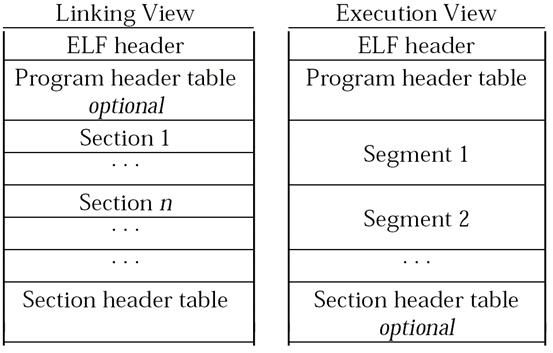
\includegraphics[scale=1]{res/lin_001}
 \caption{Структура ELF-формат с точки зрения линкера (слева) и системного загрузчика операционной системы (справа)}
\end{figure}

\subsection{Структура и назначение полей служебных заголовков}

Заголовок файла (ELF Header) имеет фиксированное расположение в начале файла и содержит общее описание структуры файла и его основные характеристики, такие как: тип, версия формата, архитектура процессора, виртуальный адрес точки входа, размеры и смещения остальных частей файла.

\begin{itemize}
\item{ \textit{e\_ident[]} -- Массив байт, каждый из которых определяет общую характеристику файла. Первые четыре байта в массиве определяют сигнатуру файла и всегда должны содержать 0x7f 0x45 0x4c 0x46 соответственно.}
\item{ \textit{e\_type} -- Тип файла.}
\item{ \textit{e\_machine} -- Архитектура аппаратной платформы, для которой файл создан.}
\item{ \textit{e\_version} -- Номер версии формата.}
\item{ \textit{e\_entry} -- Точка входа.}
\item{ \textit{e\_phoff} -- Расположение таблицы заголовков программы.}
\item{ \textit{e\_shoff} -- Расположение таблицы заголовков разделов.}
\item{ \textit{e\_flags} -- Связанные с файлом флаги, зависящие от процессора.}
\item{ \textit{e\_ehsize} -- Размер[5] заголовка файла.}
\item{ \textit{e\_phentsize} -- Размер каждого заголовка программы.}
\item{ \textit{e\_phnum} -- Число заголовков программы.}
\item{ \textit{e\_shentsize} -- Размер каждого заголовка разделов.}
\item{ \textit{e\_shnum} -- Число заголовков разделов.}
\item{ \textit{e\_shstrndx} -- Индекс записи в таблице разделов, указывающей на таблицу названий разделов.}
\end{itemize}

\subsection{Процесс загрузки в память}

По умолчанию ELF-заголовок проецируется по адресу 8048000h, который прописан в его заголовке. Это и есть базовый адрес загрузки. На стадии линковки он может быть свободно изменен на другой, но большинство программистов оставляют его как есть. Все сегменты проецируются в память в соответствии с виртуальными адресами, прописанными в таблице сегментов, причем, виртуальная проекция образа всегда непрерывна, и между сегментами не должно быть незаполненных дыр.

Начиная с адреса 40000000h располагаются совместно используемые библиотеки ld-linix.so, libm.so, libc.so и другие, которые связывают операционную систему с прикладной программой. Ближайший аналог из мира Windows -- KERENL32.DLL, реализующая win32 API, что расшифровывается как Application Programming Interface, но при желании программа может вызывать функции операционной системы и напрямую. В NT за это отвечает прерывание INT 2Eh, в LINUX -- как правило INT 80h (на самом деле к текущему моменту в этом вопросе была проделана некоторая оптимизация, о которой будет сказано позже, при рассмотрении вывода утилиты ldd)\cite{Cit3}.

Для вызова функций типа открытия файла мы можем обратиться либо к библиотеке libc, либо непосредственно к самой операционной системе. Первый вариант -- самый громоздкий, самый переносимый, и наименее приметный. Последний -- прост в реализации, но испытывает проблемы совместимости с различными версиями LINUX'а.

Последний гигабайт адресного пространства (от адреса C0000000h и выше) занимают код и данные операционной системе, к которым можно обращаться только посредством прерывания INT 80h или через разделяемые библиотеки.

Стек находится в нижних адресах. Он начинается с базового адреса загрузки и растет вверх по направлению к нулевым адресам. В большинстве Линукс-систем стек исполняем (то есть сюда можно скопировать машинный код и передать на него управления), однако, некоторые администраторы устанавливают заплатки, отнимающие у стека атрибут исполнимости. Карта памяти представлена на рисунке 2.


\begin{figure}[H]
 \centering
 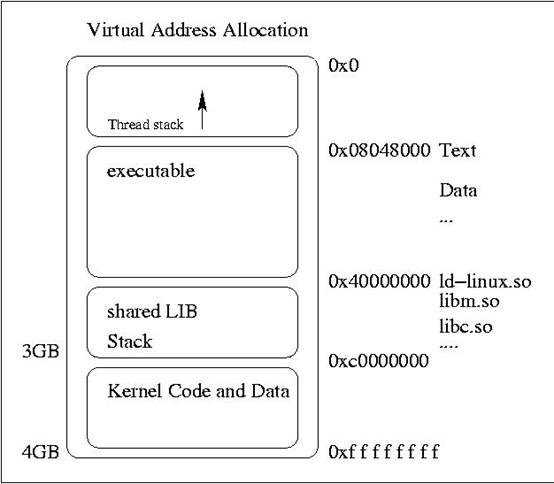
\includegraphics[scale=1]{res/lin_002}
 \caption{Карта памяти загруженного образа исполняемого файла}
\end{figure}

\subsection{Резидентное приложение -- монитор сетевой активности}

В качестве полезного приложение было решено создать простую утилиту, которая отображает количество полученных и отправленных пакетов по указанному сетевому интерфейсу. Процесс организации интерфейса с пользователем интереса не представляет, но работа с системой построена по средствам извлечения информации из файла /proc/net/dev и представлена в листинге 1.

\lstinputlisting[language=C++, firstnumber=7, firstline=7, lastline=50, caption={Функция получения информации о трафике по сетевому интерфейсу (src/ELF/lin/parse.cpp)}]
{../../src/ELF/lin/parse.cpp}

После компиляции можно собрать информацию об объектном файле. Полная демонстрация возможностей objdump займёт довольно много места, но основные возможности представлены в следующем листинге 2. В 1-й строке запрашивается информация о хедерах файла, их именах и расположении.

\lstinputlisting[language={},caption={Демонстрация работы программы objdump}]{res/objdump.output}

Другой удобной программой для вывода информации о ELF файле является readelf (вывод программы приведён в сокращенном виде, листинг 3).

\lstinputlisting[language={}, firstnumber=89, firstline=89, caption={Демонстрация работы программы readelf}]{res/readelf.output}

Информацию о символах можем получить при помощи утилиты ss (нас интересует функция parse, строка 56, листинг 4).

\lstinputlisting[language={}, firstnumber=40, firstline=40, lastline=68, caption={Демонстрация работы программы nm}]{res/nm.output}

Зависимость от библиотек показывает утилита ldd (листинг 5). Тут стоит обратить внимание на виртуальную библиотеку в строке 1. В те времена, когда процессоры с архитектурой x86 только появились, взаимодействие пользовательских приложений со службами операционной системы осуществлялось с помощью прерываний. По мере создания более мощных процессоров эта схема взаимодействия становилась узким местом системы. Во всех процессорах, начиная с Pentium II, Intel реализовала механизм быстрых системных вызовов (Fast System Call), в котором вместо прерываний используются инструкции SYSENTER и SYSEXIT, ускоряющие выполнение системных вызовов.

Библиотека linux-vdso.so.1 является виртуальной библиотекой, или виртуальным динамически разделяемым объектом (VDSO), который размещается только в адресном пространстве отдельной программы. В более ранних системах эта библиотека называлась linux-gate.so.1. Эта виртуальная библиотека содержит всю необходимую логику, обеспечивающую для пользовательских приложений наиболее быстрый доступ к системным функциям в зависимости от архитектуры процессора -- либо через прерывания, либо (для большинства современных процессоров) через механизм быстрых системных вызовов.

\lstinputlisting[language={}, caption={Демонстрация работы программы ldd}]{res/ldd.output}

Адрес загрузки программы не меняется, однако адреса подключения динамических библиотек и область размещения стека изменяются при повторном запуске. Отсюда можно сделать вывод о том, что представленные адреса виртуальные.

Теперь программу можно запустить для проверки сетевого интерфейса каждые 2 секунды. Работа программы показана на рисунке 3.

\begin{figure}[H]
 \centering
 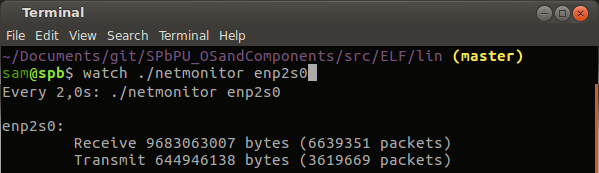
\includegraphics[scale=0.85]{res/lin_003}
 \caption{Исполнение программы}
\end{figure}

\subsection{Динамические библиотеки .so}

Библиотека - это набор скомпонованных особым образом объектных файлов. Библиотеки подключаются к основной программе во время линковки. По способу компоновки библиотеки подразделяют на архивы (статические библиотеки, static libraries) и совместно используемые (динамические библиотеки, shared libraries). В Linux, кроме того, есть механизмы динамической подгрузки библиотек. Суть динамической подгрузки состоит в том, что запущенная программа может по собственному усмотрению подключить к себе какую-либо библиотеку. Благодаря этой возможности создаются программы с подключаемыми плагинами, такие как XMMS.

Статическая библиотека - это просто архив объектных файлов, который подключается к программе во время линковки. Эффект такой же, как при компиляции файлов отдельно.

В отличие от статических библиотек, код совместно используемых (динамических) библиотек не включается в бинарник. Вместо этого в бинарник включается только ссылка на библиотеку.

Рассмотрим преимущества и недостатки статических и совместно используемых библиотек. Статические библиотеки делают программу более автономной: программа, скомпонованная со статической библиотекой может запускаться на любом компьютере, не требуя наличия этой библиотеки (она уже "внутри" бинарника). Программа, скомпонованная с динамической библиотекой, требует наличия этой библиотеки на том компьютере, где она запускается, поскольку в бинарнике не код, а ссылка на код библиотеки. Не смотря на такую зависимость, динамические библиотеки обладают двумя существенными преимуществами. Во-первых, бинарник, скомпонованный с совместно используемой библиотекой меньше размером, чем такой же бинарник, с подключенной к нему статической библиотекой (статически скомпонованный бинарник). Во-вторых, любая модернизация динамической библиотеки, отражается на всех программах, использующих ее. Таким образом, если некоторую библиотеку foo используют 10 программ, то исправление какой-нибудь ошибки в foo или любое другое улучшение библиотеки автоматически улучшает все программы, которые используют эту библиотеку. Именно поэтому динамические библиотеки называют совместно используемыми. Чтобы применить изменения, внесенные в статическую библиотеку, нужно пересобрать все 10 программ.

В Linux статические библиотеки обычно имеют расширение .a (Archive), а совместно используемые библиотеки имеют расширение .so (Shared Object). Хранятся библиотеки, как правило, в каталогах /lib и /usr/lib. В случае иного расположения (относится только к совместно используемым библиотекам), приходится явно указать путь, чтобы программа запустилась\cite{Cit2}. 

\subsection{Резидентное приложение с динамической библиотекой}

В динамическую библиотеку вынесена функция, отвечающая за взаимодействие с системой.

При компиляции, отдельно собирается библиотека, и отдельно исполняемый файл.

\begin{Verbatim}[frame=single]
user@host$ g++ -o libparse.so -shared -fPIC -std=c++14 parse.cpp
user@host$ g++ main.cpp -L. -lparse -o netmonitor
\end{Verbatim}

Теперь простой запуск приложения приведёт к ошибке, т.к. система ожидает наличия файла библиотеки в строго определённом месте.

\begin{Verbatim}[frame=single]
user@host$ ./netmonitor 
./netmonitor: error while loading shared libraries: libparse.so: cannot open shared object file: No such file or directory
user@host$
\end{Verbatim}

Отсутствие библиотеки можно легко обнаружить при запуске утилиты ldd (строка 2, листинг 6).

\lstinputlisting[language={}, caption={Демонстрация работы программы ldd для приложения, использующего динамическую библиотеку}]{res/ldd2.output}

Эту проблему можно обойти если явным образом перед запуском программы передать путь к библиотеке через параметры

\begin{Verbatim}[frame=single]
user@host$ LD_LIBRARY_PATH=. ./netmonitor enp2s0
enp2s0:
        Receive 9686554269 bytes (6645253 packets)
        Transmit 645757402 bytes (3625776 packets)
user@host$
\end{Verbatim}

Из результатов анализа распределения памяти можно сделать вывод о том, что при запуске программы ей выделяется свободное место в памяти, в следствии чего адреса, по которым располагаются точки входа или подключения меняются при повторных запусках, однако, состав, порядок и смещения загружаемых модулей относительно начального адреса в выделенной памяти не изменяется.